
\subsection{Answers}
\begin{table}[htb]%
\begin{center}%
\caption{Q16: Which MPI features have you never heard of?}%
\label{tab:Q16-ans}%
\begin{tabular}{l|l|r}%
\hline%
Choice & Abbrv. & \# Answers \\%
\hline%
PMPI interface & PMPI & 465 (66.1\%) \\%
Persistent communication & Persistent & 433 (61.5\%) \\%
Dynamic process creation & Dynamic process & 383 (54.4\%) \\%
One-sided communications & One-sided & 131 (18.6\%) \\%
{\small Communicator operations (split, duplicat$\cdots$} & Communicator & 123 (17.5\%) \\%
Point-to-point communications & Point-to-point & 91 (12.9\%) \\%
MPI datatypes & Datatypes & 90 (12.8\%) \\%
Collective communications & Collectives & 86 (12.2\%) \\%
MPI with OpenMP (or multithread) & with OpenMP & 86 (12.2\%) \\%
\hline%
\multicolumn{2}{c}{total} & 1888 (704)\\%
\hline%
\end{tabular}%
\end{center}%
\end{table}%

\clearpage%
{\footnotesize\begin{landscape}%
\begin{longtable}[htb]{r|c|c|c|c|c|c|c|c|c|c}%
\caption{Q16: Which MPI features have you never heard of?}%
\label{tab:Q16-mans} \\%
\hline%
Multi-Answer & overall & FR & GR & IT & UK & eu & JP & RU & US & others \\
 \hline%
\endfirsthead%
\multicolumn{11}{r}{(continued from the previous page)}\\%
\hline%
Multi-Answer & overall & FR & GR & IT & UK & eu & JP & RU & US & others \\
 \hline%
\endhead%
\hline%
(total) & 704 & 103 & 131 & 52 & 58 & 119 & 50 & 86 & 33 & 72 \\%
\hline%
\multicolumn{11}{r}{(continue to the next page)}\\%
\endfoot%
\hline%
(total) & 704 & 103 & 131 & 52 & 58 & 119 & 50 & 86 & 33 & 72 \\%
\hline%
\endlastfoot%
\hline%
{Dyn. process, Persistent, PMPI} & 126 & 13 & 33 & 16 & 9 & 23 & 6 & 14 & 3 & 9 \\%
{PMPI} & 84 & 14 & 20 & 5 & 6 & 12 & 5 & 11 & 5 & 6 \\%
{Persistent} & 65 & 7 & 16 & 3 & 11 & 9 & 8 & 3 & 2 & 6 \\%
{Persistent, PMPI} & 62 & 7 & 9 & 0 & 4 & 10 & 6 & 15 & 3 & 8 \\%
{Dyn. process, Persistent} & 43 & 5 & 8 & 6 & 5 & 7 & 6 & 2 & 2 & 2 \\%
{Dyn. process} & 38 & 9 & 8 & 1 & 0 & 8 & 3 & 2 & 3 & 4 \\%
{Dyn. process, PMPI} & 32 & 8 & 6 & 2 & 3 & 3 & 0 & 3 & 5 & 2 \\%
{One-sided, Dyn. process, Persistent, PMPI} & 30 & 5 & 2 & 4 & 3 & 10 & 1 & 3 & 0 & 2 \\%
{Communicator, Dyn. process, Persistent, PMPI} & 16 & 4 & 2 & 1 & 3 & 2 & 0 & 2 & 0 & 2 \\%
{Communicator, Dyn. process, PMPI} & 11 & 2 & 2 & 1 & 2 & 2 & 0 & 2 & 0 & 0 \\%
{Point-to-point, Collectives, Communicator, Datatypes, One-sided, with OpenMP} & 11 & 0 & 3 & 0 & 1 & 4 & 1 & 0 & 1 & 1 \\%
{Point-to-point, Collectives, Communicator, Datatypes, One-sided, Dyn. process, Persistent, with OpenMP, PMPI} & 9 & 3 & 1 & 0 & 2 & 1 & 1 & 1 & 0 & 0 \\%
{One-sided, PMPI} & 8 & 1 & 1 & 0 & 1 & 0 & 2 & 0 & 0 & 3 \\%
{with OpenMP} & 8 & 1 & 1 & 0 & 0 & 0 & 1 & 1 & 1 & 3 \\%
{Point-to-point, Collectives, Communicator, Datatypes, One-sided, Dyn. process, Persistent, PMPI} & 7 & 1 & 0 & 0 & 0 & 6 & 0 & 0 & 0 & 0 \\%
{One-sided, Dyn. process, Persistent} & 6 & 2 & 1 & 0 & 0 & 0 & 0 & 2 & 0 & 1 \\%
{Point-to-point, Collectives, Datatypes, with OpenMP} & 6 & 1 & 2 & 1 & 0 & 1 & 0 & 0 & 1 & 0 \\%
{One-sided, Persistent, PMPI} & 5 & 1 & 1 & 0 & 1 & 1 & 0 & 1 & 0 & 0 \\%
{Communicator, One-sided, Dyn. process, Persistent, PMPI} & 5 & 0 & 3 & 0 & 0 & 0 & 0 & 0 & 0 & 2 \\%
{Communicator, Persistent, PMPI} & 4 & 0 & 0 & 0 & 0 & 0 & 2 & 1 & 0 & 1 \\%
{Point-to-point, Collectives, Communicator, Datatypes} & 4 & 1 & 1 & 1 & 0 & 0 & 0 & 0 & 1 & 0 \\%
{One-sided, Dyn. process, Persistent, with OpenMP, PMPI} & 4 & 0 & 2 & 0 & 0 & 1 & 0 & 1 & 0 & 0 \\%
{Point-to-point} & 4 & 0 & 0 & 0 & 0 & 0 & 0 & 2 & 0 & 2 \\%
{with OpenMP, PMPI} & 4 & 0 & 0 & 0 & 0 & 0 & 0 & 0 & 1 & 3 \\%
{Point-to-point, Collectives, Communicator, Datatypes, One-sided, Dyn. process, Persistent, with OpenMP} & 3 & 1 & 0 & 1 & 0 & 1 & 0 & 0 & 0 & 0 \\%
{Persistent, with OpenMP, PMPI} & 3 & 1 & 0 & 0 & 0 & 0 & 0 & 2 & 0 & 0 \\%
{Datatypes, PMPI} & 3 & 1 & 0 & 0 & 0 & 1 & 0 & 1 & 0 & 0 \\%
{Point-to-point, Collectives, Datatypes, One-sided, with OpenMP} & 3 & 1 & 1 & 1 & 0 & 0 & 0 & 0 & 0 & 0 \\%
{Point-to-point, Collectives} & 3 & 0 & 0 & 0 & 0 & 0 & 1 & 1 & 0 & 1 \\%
{Datatypes} & 3 & 0 & 0 & 0 & 0 & 0 & 0 & 1 & 0 & 2 \\%
{Point-to-point, Collectives, Communicator, Datatypes, with OpenMP} & 3 & 0 & 0 & 0 & 0 & 2 & 0 & 0 & 0 & 1 \\%
{Point-to-point, Collectives, Communicator, Datatypes, One-sided, Persistent, with OpenMP, PMPI} & 3 & 0 & 1 & 1 & 0 & 0 & 0 & 0 & 1 & 0 \\%
{Communicator, PMPI} & 3 & 1 & 0 & 0 & 0 & 1 & 0 & 1 & 0 & 0 \\%
{Communicator} & 3 & 0 & 0 & 0 & 0 & 0 & 0 & 1 & 1 & 1 \\%
{Dyn. process, with OpenMP, PMPI} & 3 & 0 & 0 & 0 & 0 & 0 & 1 & 2 & 0 & 0 \\%
{Point-to-point, Dyn. process, Persistent, PMPI} & 3 & 0 & 0 & 1 & 0 & 0 & 1 & 0 & 0 & 1 \\%
{Datatypes, Dyn. process, PMPI} & 3 & 1 & 0 & 0 & 0 & 1 & 1 & 0 & 0 & 0 \\%
{Point-to-point, Collectives, Communicator, Datatypes, One-sided, with OpenMP, PMPI} & 3 & 0 & 0 & 1 & 0 & 1 & 0 & 1 & 0 & 0 \\%
{Persistent, with OpenMP} & 2 & 2 & 0 & 0 & 0 & 0 & 0 & 0 & 0 & 0 \\%
{Point-to-point, Collectives, Communicator, Datatypes, Dyn. process, Persistent, with OpenMP} & 2 & 1 & 0 & 0 & 1 & 0 & 0 & 0 & 0 & 0 \\%
{Communicator, One-sided, Dyn. process, Persistent} & 2 & 0 & 1 & 0 & 0 & 0 & 0 & 1 & 0 & 0 \\%
{Point-to-point, Collectives, Communicator, Datatypes, One-sided, Dyn. process, with OpenMP} & 2 & 0 & 0 & 0 & 0 & 1 & 1 & 0 & 0 & 0 \\%
{Communicator, Datatypes, One-sided, Dyn. process, Persistent, PMPI} & 2 & 0 & 0 & 0 & 1 & 0 & 0 & 1 & 0 & 0 \\%
{One-sided, Dyn. process, PMPI} & 2 & 0 & 0 & 0 & 0 & 1 & 0 & 0 & 0 & 1 \\%
{Collectives} & 2 & 1 & 0 & 0 & 0 & 0 & 0 & 1 & 0 & 0 \\%
{Point-to-point, Collectives, Communicator, One-sided, Dyn. process, Persistent, PMPI} & 2 & 0 & 0 & 0 & 1 & 0 & 0 & 0 & 0 & 1 \\%
{Point-to-point, Persistent, PMPI} & 2 & 0 & 0 & 0 & 0 & 0 & 1 & 1 & 0 & 0 \\%
{Point-to-point, One-sided, Dyn. process, Persistent, PMPI} & 2 & 1 & 1 & 0 & 0 & 0 & 0 & 0 & 0 & 0 \\%
{Communicator, Dyn. process} & 2 & 1 & 0 & 0 & 0 & 0 & 1 & 0 & 0 & 0 \\%
{Datatypes, Dyn. process, Persistent, PMPI} & 2 & 0 & 0 & 1 & 0 & 0 & 0 & 0 & 0 & 1 \\%
{Dyn. process, Persistent, with OpenMP, PMPI} & 2 & 0 & 0 & 0 & 1 & 1 & 0 & 0 & 0 & 0 \\%
{One-sided} & 2 & 0 & 0 & 0 & 0 & 0 & 0 & 0 & 1 & 1 \\%
{Datatypes, Persistent, PMPI} & 2 & 2 & 0 & 0 & 0 & 0 & 0 & 0 & 0 & 0 \\%
{Point-to-point, Communicator, One-sided, Dyn. process, Persistent, with OpenMP, PMPI} & 1 & 1 & 0 & 0 & 0 & 0 & 0 & 0 & 0 & 0 \\%
{Point-to-point, Communicator, Dyn. process, Persistent, PMPI} & 1 & 0 & 0 & 0 & 0 & 1 & 0 & 0 & 0 & 0 \\%
{Point-to-point, Communicator, Dyn. process, Persistent} & 1 & 0 & 0 & 1 & 0 & 0 & 0 & 0 & 0 & 0 \\%
{Collectives, Communicator, Datatypes, with OpenMP} & 1 & 0 & 0 & 0 & 0 & 0 & 0 & 1 & 0 & 0 \\%
{Collectives, Datatypes, Dyn. process, PMPI} & 1 & 0 & 0 & 0 & 0 & 1 & 0 & 0 & 0 & 0 \\%
{Point-to-point, Collectives, Communicator, Datatypes, One-sided, Dyn. process, Persistent} & 1 & 0 & 1 & 0 & 0 & 0 & 0 & 0 & 0 & 0 \\%
{Point-to-point, Collectives, Communicator, Dyn. process, PMPI} & 1 & 0 & 0 & 0 & 0 & 1 & 0 & 0 & 0 & 0 \\%
{Dyn. process, with OpenMP} & 1 & 0 & 0 & 0 & 0 & 0 & 0 & 0 & 1 & 0 \\%
{Collectives, Communicator, Datatypes, One-sided, Dyn. process, Persistent, PMPI} & 1 & 0 & 1 & 0 & 0 & 0 & 0 & 0 & 0 & 0 \\%
{Communicator, Datatypes, Dyn. process, Persistent} & 1 & 0 & 0 & 0 & 0 & 0 & 0 & 0 & 0 & 1 \\%
{Point-to-point, Datatypes, One-sided, Dyn. process, Persistent} & 1 & 0 & 0 & 0 & 0 & 0 & 0 & 1 & 0 & 0 \\%
{Point-to-point, Collectives, Communicator, Datatypes, Dyn. process, with OpenMP} & 1 & 0 & 0 & 0 & 0 & 1 & 0 & 0 & 0 & 0 \\%
{Communicator, One-sided, Dyn. process, PMPI} & 1 & 0 & 0 & 0 & 1 & 0 & 0 & 0 & 0 & 0 \\%
{Collectives, Datatypes, One-sided, with OpenMP} & 1 & 0 & 0 & 0 & 0 & 1 & 0 & 0 & 0 & 0 \\%
{Communicator, One-sided, Dyn. process, with OpenMP, PMPI} & 1 & 0 & 0 & 0 & 1 & 0 & 0 & 0 & 0 & 0 \\%
{Point-to-point, Datatypes, One-sided, Dyn. process, Persistent, PMPI} & 1 & 1 & 0 & 0 & 0 & 0 & 0 & 0 & 0 & 0 \\%
{Collectives, Communicator, One-sided, Dyn. process, Persistent, PMPI} & 1 & 0 & 0 & 0 & 0 & 0 & 0 & 0 & 0 & 1 \\%
{Point-to-point, Collectives, Datatypes, One-sided, Dyn. process, with OpenMP} & 1 & 0 & 0 & 0 & 1 & 0 & 0 & 0 & 0 & 0 \\%
{Collectives, Datatypes} & 1 & 0 & 0 & 0 & 0 & 0 & 0 & 1 & 0 & 0 \\%
{Collectives, Communicator, with OpenMP} & 1 & 0 & 1 & 0 & 0 & 0 & 0 & 0 & 0 & 0 \\%
{Point-to-point, Collectives, Datatypes} & 1 & 0 & 0 & 0 & 0 & 0 & 0 & 0 & 0 & 1 \\%
{Point-to-point, Collectives, Communicator, Datatypes, One-sided, Persistent, with OpenMP} & 1 & 1 & 0 & 0 & 0 & 0 & 0 & 0 & 0 & 0 \\%
{One-sided, Persistent} & 1 & 0 & 0 & 0 & 0 & 0 & 1 & 0 & 0 & 0 \\%
{Communicator, One-sided, Dyn. process} & 1 & 0 & 0 & 0 & 0 & 1 & 0 & 0 & 0 & 0 \\%
{Point-to-point, Collectives, Communicator, with OpenMP} & 1 & 0 & 0 & 0 & 0 & 1 & 0 & 0 & 0 & 0 \\%
{One-sided, with OpenMP, PMPI} & 1 & 0 & 0 & 0 & 0 & 1 & 0 & 0 & 0 & 0 \\%
{Point-to-point, Collectives, Communicator, Datatypes, One-sided, Dyn. process, PMPI} & 1 & 0 & 0 & 0 & 0 & 1 & 0 & 0 & 0 & 0 \\%
{Point-to-point, Collectives, Communicator, Datatypes, One-sided, Dyn. process, with OpenMP, PMPI} & 1 & 0 & 0 & 0 & 0 & 0 & 0 & 1 & 0 & 0 \\%
{Collectives, Dyn. process, Persistent} & 1 & 0 & 0 & 1 & 0 & 0 & 0 & 0 & 0 & 0 \\%
{Point-to-point, Communicator, Datatypes, One-sided, Persistent} & 1 & 0 & 0 & 0 & 0 & 0 & 0 & 0 & 1 & 0 \\%
{Point-to-point, Collectives, with OpenMP} & 1 & 0 & 0 & 1 & 0 & 0 & 0 & 0 & 0 & 0 \\%
{Point-to-point, Collectives, Datatypes, One-sided} & 1 & 0 & 0 & 0 & 0 & 0 & 0 & 1 & 0 & 0 \\%
{Point-to-point, Collectives, Communicator, One-sided, Dyn. process, PMPI} & 1 & 0 & 0 & 0 & 0 & 0 & 0 & 0 & 0 & 1 \\%
{Collectives, Datatypes, PMPI} & 1 & 0 & 0 & 1 & 0 & 0 & 0 & 0 & 0 & 0 \\%
{Point-to-point, Collectives, Communicator, Dyn. process, Persistent, PMPI} & 1 & 0 & 0 & 0 & 0 & 0 & 0 & 0 & 0 & 1 \\%
{Communicator, Dyn. process, Persistent} & 1 & 0 & 1 & 0 & 0 & 0 & 0 & 0 & 0 & 0 \\%
{Collectives, Communicator, Persistent, with OpenMP, PMPI} & 1 & 0 & 0 & 1 & 0 & 0 & 0 & 0 & 0 & 0 \\%
{Communicator, Datatypes, One-sided, Persistent, PMPI} & 1 & 0 & 0 & 0 & 0 & 0 & 0 & 1 & 0 & 0 \\%
{Communicator, Persistent} & 1 & 1 & 0 & 0 & 0 & 0 & 0 & 0 & 0 & 0 \\%
{Communicator, Dyn. process, Persistent, with OpenMP, PMPI} & 1 & 0 & 1 & 0 & 0 & 0 & 0 & 0 & 0 & 0 \\%
\hline%
\end{longtable}%
\end{landscape}}%
\clearpage%


\begin{figure}[htb]
\begin{center}
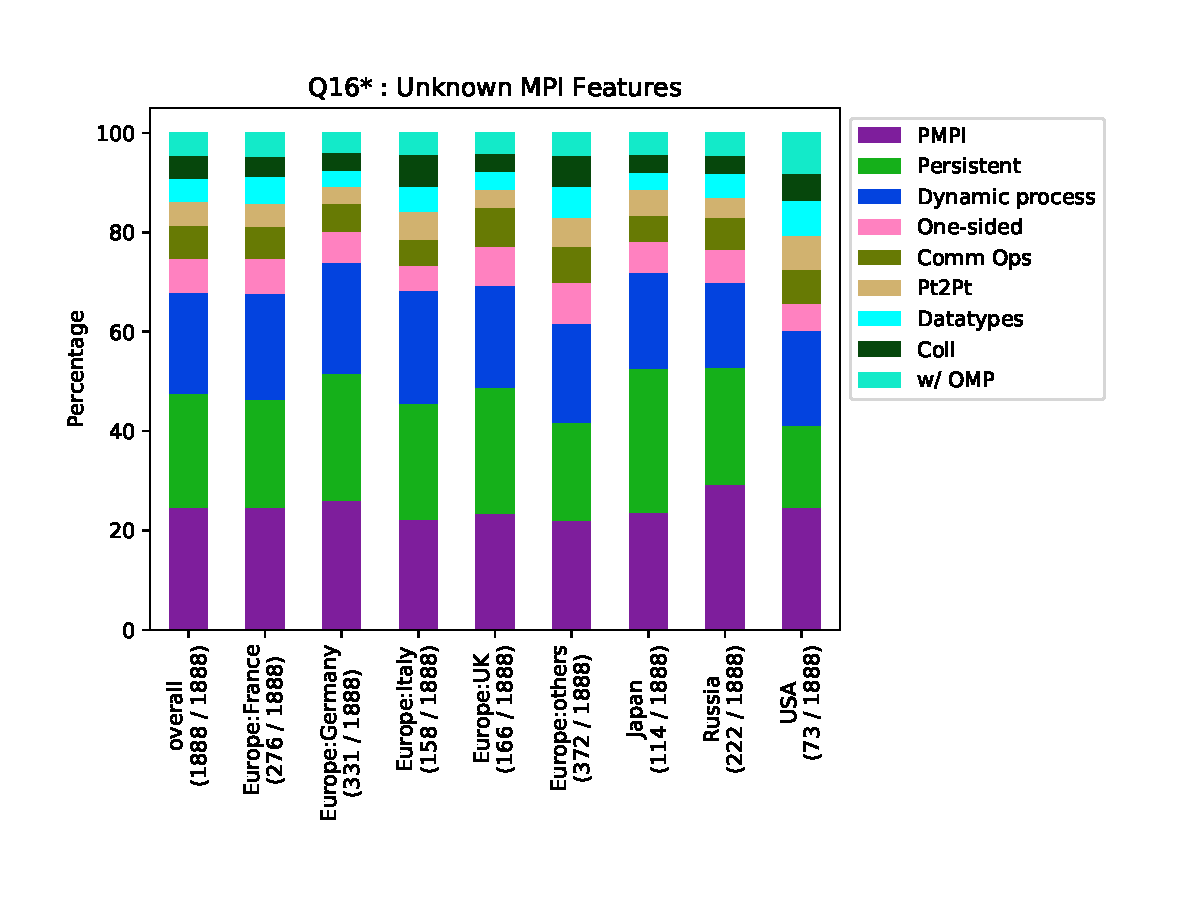
\includegraphics[width=10cm]{../pdfs/Q16.pdf}
\caption{Simple analysis: Q16}
\label{fig:Q16}
\end{center}
\end{figure}

\subsection{Comments}

There are some MPI features that are not well-known because they are very
specific and/or difficult to use. This is the case for PMPI (that can be used for
debugging), persistent communication (used to optimize repeated communication),
and dynamic process creation (useful when the number of processes varies during
execution). These features represent around  60 \% of the answers showing that
they are very specific. The other answers represent less that 7\% of the
total.  For this question, it is hard to see any difference region-wise.
